% ******************************************************** %
% DOCUMENT INFORMATION                                     %
% ******************************************************** %
%                                                          %
%                                                          %
% Purpose of Document                                      %
% -------------------                                      %
% Technical Report                                         %
%                                                          %
% Institution                                              %
% -----------                                              %
% University of Applied Sciences and Arts Northwestern     %
% Switzerland, School of Engineering                       %
%                                                          %
% Degree Program                                           %
% --------------                                           %
% Electrical Engineering and Information Technology, BSc.  %
%                                                          %
% Course                                                   %
% ------                                                   %
% Project 5, Fall Semester 2016                            %
%                                                          %
% Authors                                                  %
% -------                                                  %
% Raphael Frey                                             %
% Alex Murray                                              %
%                                                          %
% Document Design and Maintenance                          %
% -------------------------------                          %
% Raphael Frey                                             %
% Based on my own work. The  template on which this report %
% was based is available at:                               %
% https://github.com/alpenwasser/longtex                   %
% -------------------------------------------------------- %

\documentclass[11pt, a4paper, oneside]{memoir}

% -------------------------------------------------------- %
% Different font and pages  sizes, layouts. Not a complete %
% list, just what I've used on occasion.                   %
% -------------------------------------------------------- %
%\documentclass[9pt,b5paper]{memoir}
%\documentclass[twocolumn,9pt,a4paper]{memoir}
%\documentclass[10pt,a5paper]{memoir} % ~60 chars per line
%\documentclass[12pt,a4paper]{memoir} % ~60 to 70 chars per line


% -------------------------------------------------------- %
% Preamble  stuff  is  kept in  the  preamble/  directory, %
% separated  out into  different files  as needed  to keep %
% things modular.                                          %
% -------------------------------------------------------- %
% -------------------------------------------------------- %
% NOTE: There   are  two   kinds  of   packages  in   this %
% document. On ond hand, there  are those which are needed %
% for this  template to function at  as intended. It might %
% still  compile without  them,  but it  will probably  no %
% longer look as it should.                                %
%                                                          %
% On the other hand, there are those which I have found to %
% be useful over the years  and tend to commonly use.  You %
% may or may  not need those.  Feel free  to disable those %
% you do not need.                                         %
%                                                          %
% By default,  I recommend leaving the  following packages %
% enabled:                                                 %
% - fontenc: for output font encoding                      %
% - inputenc: for using  non-standard characters in input, %
%   such as Umlauts or other accented characters           %
% - graphicx:  needed for  the  chapter  style (based  on  %
%   veelo)                                                 %
%                                                          %
% Feel free to  disable and enable the  rest as needed. If %
% the document no longer compiles or breaks aesthetically, %
% you will notice soon enough...                           %
% -------------------------------------------------------- %


% -------------------------------------------------------- %
% General Packages                                         %
% -------------------------------------------------------- %
\usepackage[T1]{fontenc}     % output encoding
\usepackage[utf8]{inputenc}  % input encoding
\usepackage[ngerman]{babel}
\usepackage{lipsum}          % filler text
\usepackage{graphicx}
\usepackage{amsmath}         % for reasonable math typesetting
\usepackage{pdfpages}        % include pdf documents
%\usepackage{amsfonts}        % not sure yet if we need this
\usepackage{adjustbox}       % helps w/ minipage alignmant
\usepackage[textsize=footnotesize, textwidth = 37mm, german, colorinlistoftodos]{todonotes}
\usepackage{calc}            % used for calculating margins and widths for A3 pages
%\usepackage{caption}         % captions outside float environments, overrides memoir's caption facilities
\usepackage[separate-uncertainty=true]{siunitx}
\usepackage[light]{kpfonts}
\usepackage{counttexruns}
\usepackage[european,siunitx,cuteinductors]{circuitikz}


% -------------------------------------------------------- %
% Draft Watermark                                          %
%                                                          %
% Prints  a watermark  across the  page, marking  it as  a %
% draft.                                                   %
% -------------------------------------------------------- %
\usepackage{draftwatermark}
\SetWatermarkText{Entwurf, \today}
\SetWatermarkScale{0.5}
%\usepackage[final]{draftwatermark} % removes watermark



% -------------------------------------------------------- %
% TIKZ and PGF                                             %
%                                                          %
% TODO: See if this  should be put in a  separate file, or %
% if  having  it  here makes  sense. Alternatively,  these %
% documents might not need to be set globally at all.      %
% -------------------------------------------------------- %
\usepackage{tikz}
\usetikzlibrary{arrows}
\usetikzlibrary{decorations.pathmorphing}
\usepackage{pgfplots}
\pgfplotsset{compat=newest}
\pgfplotsset{max space between ticks=80pt}
\pgfplotsset{max space between ticks=80pt}
\pgfplotsset{try min ticks=5}
\pgfplotsset{
    tick label style={font=\small},
    label style={font=\small},
    legend style={font=\footnotesize}
}


% -------------------------------------------------------- %
% Conditionals                                             %
% -------------------------------------------------------- %
% http://tex.stackexchange.com/questions/5894/latex-conditional-expression
\usepackage{etoolbox}

% -------------------------------------------------------- %
% Packages which might be used under certain circumstances %
% -------------------------------------------------------- %
%\usepackage{geometry}
%\usepackage[english]{babel}
%\usepackage{kpfonts}

% -------------------------------------------------------- %
% Set link  colors and  all that good  stuff. See hyperref %
% manual for more info and options if you wish.            %
% -------------------------------------------------------- %
\newtoggle{paper}
%\toggletrue{paper} % we're printing on paper
\togglefalse{paper} % we're making an electronic version

\iftoggle{paper}{%
    % ---------------------------------------------------- %
    % If  we're  printing on  paper,  don't  do any  fancy %
    % coloring for links and such.                         %
    % ---------------------------------------------------- %
    \usepackage[%
        bookmarksnumbered=true,
        colorlinks=true,
        linkcolor=black,
        citecolor=black,
        urlcolor=black,
        %hidelinks=false,
    ]{hyperref}
}{%
    % ---------------------------------------------------- %
    % If  we're  creating  an electronic  version  of  our %
    % document, color links as follows.                    %
    % ---------------------------------------------------- %
    \usepackage[%
        bookmarksnumbered=true,
        colorlinks=true,
        linkcolor=blue,
        citecolor=blue,
        urlcolor=magenta,
        %hidelinks=false,
    ]{hyperref}
}


% -------------------------------------------------------- %
% xcolor  and kvoptions  are  loaded by  xcolor-solarized. %
% If   you  require   special   options   for  these   two %
% packages,  uncomment  these  two lines  and  pass  those %
% options. Otherwise  leave them  commented out  since the %
% packages are loaded anyway.                              %
% -------------------------------------------------------- %
%\usepackage{xcolor}
%\usepackage{kvoptions}
\usepackage{xcolor-solarized}

% -------------------------------------------------------- %
% This file contains various options for the memoir class  %
% itself.                                                  %
% -------------------------------------------------------- %


% -------------------------------------------------------- %
% Choose a page layout                                     %
% -------------------------------------------------------- %
%\isopage
\semiisopage
%\medievalpage
\checkandfixthelayout


% -------------------------------------------------------- %
% Choose a chapter style                                   %
% We're  going  with  veelo, but  removing  the  "Chapter" %
% designation in front of the chapter number.              %
% -------------------------------------------------------- %
% -------------------------------------------------------- %
% This  chapterstyle is  baesd on  veelo, but  removes the %
% "Chapter" designation in front of the chapter number.    %
% -------------------------------------------------------- %
%
% TODO: Check if this is allowed by the  LPPL, under which
% 'memoir.cls' is distributed, which contains the original
% code for the veelo chapter style.
%
% http://www.latex-project.org/lppl.txt
%
% If this is not permitted, implement alternative via this:
% http://tex.stackexchange.com/questions/51527/chapter-heading-with-the-word-chapter-replaced-by-chapter-name

\makeatletter
\makechapterstyle{fhnw}{%
   \setlength{\afterchapskip}{40pt}
  \renewcommand*{\chapterheadstart}{\vspace*{40pt}}
  \renewcommand*{\afterchapternum}{\par\nobreak\vskip 25pt}
   \renewcommand*{\chapnamefont}{\normalfont\LARGE\flushright}
   \renewcommand*{\chapnumfont}{\normalfont\HUGE}
   \renewcommand*{\chaptitlefont}{\normalfont\HUGE\bfseries\flushright}
   \renewcommand*{\printchaptername}{%
       \chapnamefont\MakeTextUppercase{}}
   \renewcommand*{\chapternamenum}{}
  \setlength{\beforechapskip}{18mm}%  \numberheight
  \setlength{\midchapskip}{\paperwidth}% \barlength
  \addtolength{\midchapskip}{-\textwidth}
  \addtolength{\midchapskip}{-\spinemargin}
   \renewcommand*{\printchapternum}{%
     \makebox[0pt][l]{%
       \hspace{.8em}%
       \resizebox{!}{\beforechapskip}{\chapnumfont \thechapter}%
       \hspace{.8em}%
       \rule{\midchapskip}{\beforechapskip}%
     }%
   }%
   \makeoddfoot{plain}{}{}{\thepage}}
\makeatother

\chapterstyle{fhnw} % requires graphicx package

\pagestyle{headings}
% -------------------------------------------------------- %
% Define  what  sort  of  sectional  divisions  should  be %
% numbered.  See also "Document Divisions -- Numbering" in %
% the memoir manual.                                       %
%                                                          %
%            Division            |  Level                  %
%          ----------------------+---------                %
%            \book               |  -2                     %
%            \part               |  -1                     %
%            \chapter            |   0                     %
%            \section            |   1                     %
%            \subsection         |   2                     %
%            \subsubsection      |   3                     %
%            \paragraph          |   4                     %
%            \subparagraph       |   5                     %
%                                                          %
% \setsecnumdepth{<division>} sets  division numberings so %
% that <division>  and above will be  numbered.  When used %
% in  the preamble  (such as  here), \setsecnumdepth  also %
% calls \maxsecnumdepth, which is the numbering level used %
% in the \mainmatter part of the document. \setsecnumdepth %
% can be used anywhere  in the mainmatter to (temporarily) %
% change the numbering level.                              %
%                                                          %
% This template  uses chapters, sections,  subsections and %
% subsubsections  by default,  so  we  will set  numbering %
% level to subsubsection per default. Adjust as needed. We %
% will set this to subsubsection per default.              %
% -------------------------------------------------------- %
\setsecnumdepth{subsubsection}
\maxsecnumdepth{subsubsection}
\settocdepth{subsubsection}
\maxtocdepth{subsubsection}

\def\code#1{\texttt{#1}}
\def\quelleVA{\emph{Quelle:} Versuchsanleitung}
\def\anweisung{\emph{Anmerkung f\"ur Autoren: }}
\def\Raspi{Raspberry Pi}


\definecolor{darkred}{rgb}{0.7,0,0}
\definecolor{darkblue}{rgb}{0.6,0.6,1}
\definecolor{darkgray}{gray}{0.4}
% checkmark
\newcommand{\checkmark}{\tikz\fill[fill=black!30!green,scale=0.4](0,.35) -- (.25,0) -- (1,.7) -- (.25,.15) -- cycle;}
% partially fulfilled
\newcommand{\partially}{\tikz\fill[fill=darkblue,scale=0.4](.5,0) -- (.55,.28) -- (.8,.33) -- (.55,.38) -- (.55,.62) -- (.8,.67) -- (.55,.72) -- (.5,1) -- (.45,.72) -- (.2,.67) -- (.45,.62) -- (.45,.38) -- (.2,.33) -- (.45,.28) -- cycle;}
% no indication
\newcommand{\noi}{\textcolor{darkgray}{\small\textsf{---}}}
% not present
\newcommand{\np}{\tikz\fill[fill=darkred,scale=0.4](0,0) -- (.5,.4) -- (1,0) -- (.6,.5) -- (1,1) -- (.5,.6) -- (0,1) -- (.4,.5) -- cycle;}
%\newcommand{\nv}{\textcolor{darkred}{$×$}}

\newcommand{\Sensor}{Sensor }
\newcommand{\Master}{Master-Ger\"at }

\newcommand{\myfancybreaksymbol}{\Diamond}
\newcommand{\myfancybreak}{\fancybreak{$\myfancybreaksymbol\quad\myfancybreaksymbol\quad\myfancybreaksymbol$}}

\newenvironment{conditions}
  {\noindent Wobei: \par\vspace{\abovedisplayskip}\noindent\begin{tabular}{>{$}l<{$} @{${}:{}$} l}}
  {\end{tabular}\par\vspace{\belowdisplayskip}}

% -------------------------------------------------------- %
% Provides  a   new  environment  a3pages   for  inserting %
% landscape a3pages at arbitrary points in your document.  %
%                                                          %
% NOTE: This environment needs to be enclosed in braces to %
% work  correctly.  Unfortunately,  I  haven't managed  to %
% integrate  those into  the commands  directly yet  (they %
% obviously mess up the bracing of the command itself).    %
%                                                          %
% EXAMPLE:                                                 %
%                                                          %
% {\begin{a3pages}                                         %
%     your content                                         %
%     goes here                                            %
%     and will be put on                                   %
%     landscape A3 pages                                   %
% \end{a3pages}}                                           %
%                                                          %
% Note the  opening brace  before \begin{a3pages}  and the %
% additional closing brace after \end{a3pages}             %
% -------------------------------------------------------- %
% See also:
% http://tex.stackexchange.com/questions/16942/difference-between-textwidth-linewidth-and-hsize

\newenvironment{a3pages}
    {%
        \clearpage
        \setlength{\pdfpagewidth}{2\pdfpagewidth}
        \setlength{\hsize}{\pdfpagewidth-\spinemargin-\foremargin} % for text paragraphs
        \setlength{\textwidth}{\hsize}                             % headers, footers
        \setlength{\stockwidth}{2\stockwidth}
        \setlength{\paperwidth}{2\paperwidth}
        \checkandfixthelayout%
    }
    {%
        \clearpage
    }



% -------------------------------------------------------- %
% If only some files are to  be included in the file for a %
% compilation run, specify those files here.               %
% -------------------------------------------------------- %
%\includeonly{%
%    frontmatter/info,
%    frontmatter/abstract,
%    mainmatter/einleitung,
%    mainmatter/uberblick,
%    mainmatter/models,
%    mainmatter/simu,
%    mainmatter/hardware,
%    mainmatter/hardware-sensor,
%    mainmatter/hardware-master,
%    mainmatter/software,
%    mainmatter/firmware-sensor,
%    mainmatter/software-master,
%    mainmatter/validierung,
%    mainmatter/userguide,
%    mainmatter/fazit,
%    appendices/commercial-modules,
%    appendices/ltspice,
%    appendices/schema,
%    appendices/validierung,
%    appendices/costs,
%    appendices/datentrager,
%}

% ******************************************************** %
\begin{document}
% ******************************************************** %
%\fontfamily{pbk}\selectfont

% -------------------------------------------------------- %
% NOTE: The titlepage will also leave one empty page after %
% itself, so that it doesn't  get its backside printed for %
% double-sided  printing. If  document  has  been  set  to %
% single-sided  printing,  no  empty verso  page  will  be %
% added.                                                   %
% -------------------------------------------------------- %
\begin{titlingpage}


    % ---------------------------------------------------- %
    % Main Info on Contents                                %
    % ---------------------------------------------------- %
    \newcommand{\infotable}{%
        \begin{tabular}{r|l}
            \textsc{\textbf{Studiengang}}
            & EIT\\
            [4mm]

            \textsc{\textbf{Modul}}
            & Projekt 4 \\
            [4mm]

            \textsc{\textbf{Team}}
            & 3 \\
            [4mm]

            \textsc{\textbf{Autoren}}
            & Marcel Heymann, Noah H\"usser, Raphael Frey, Dominik Keller,  \\
            & Marco Koch, Reto Nussbaumer, Francesco Rovelli                \\
            [4mm]

            \textsc{\textbf{Version}}
            & 0.1 \\
        \end{tabular}%
    }%


    % ---------------------------------------------------- %
    % Place the Background Picture and Info Table          %
    % ---------------------------------------------------- %
    \hspace{-2.54mm}
    \newlength{\logoX}
    \setlength{\logoX}{5mm}
    \newlength{\logoY}
    \setlength{\logoY}{5mm}
    \begin{tikzpicture}[remember picture, overlay]
        % ------------------------------------------------ %
        % Background Picture                               %
        % ------------------------------------------------ %
        \node[inner sep=0pt] at (current page.center) {%
            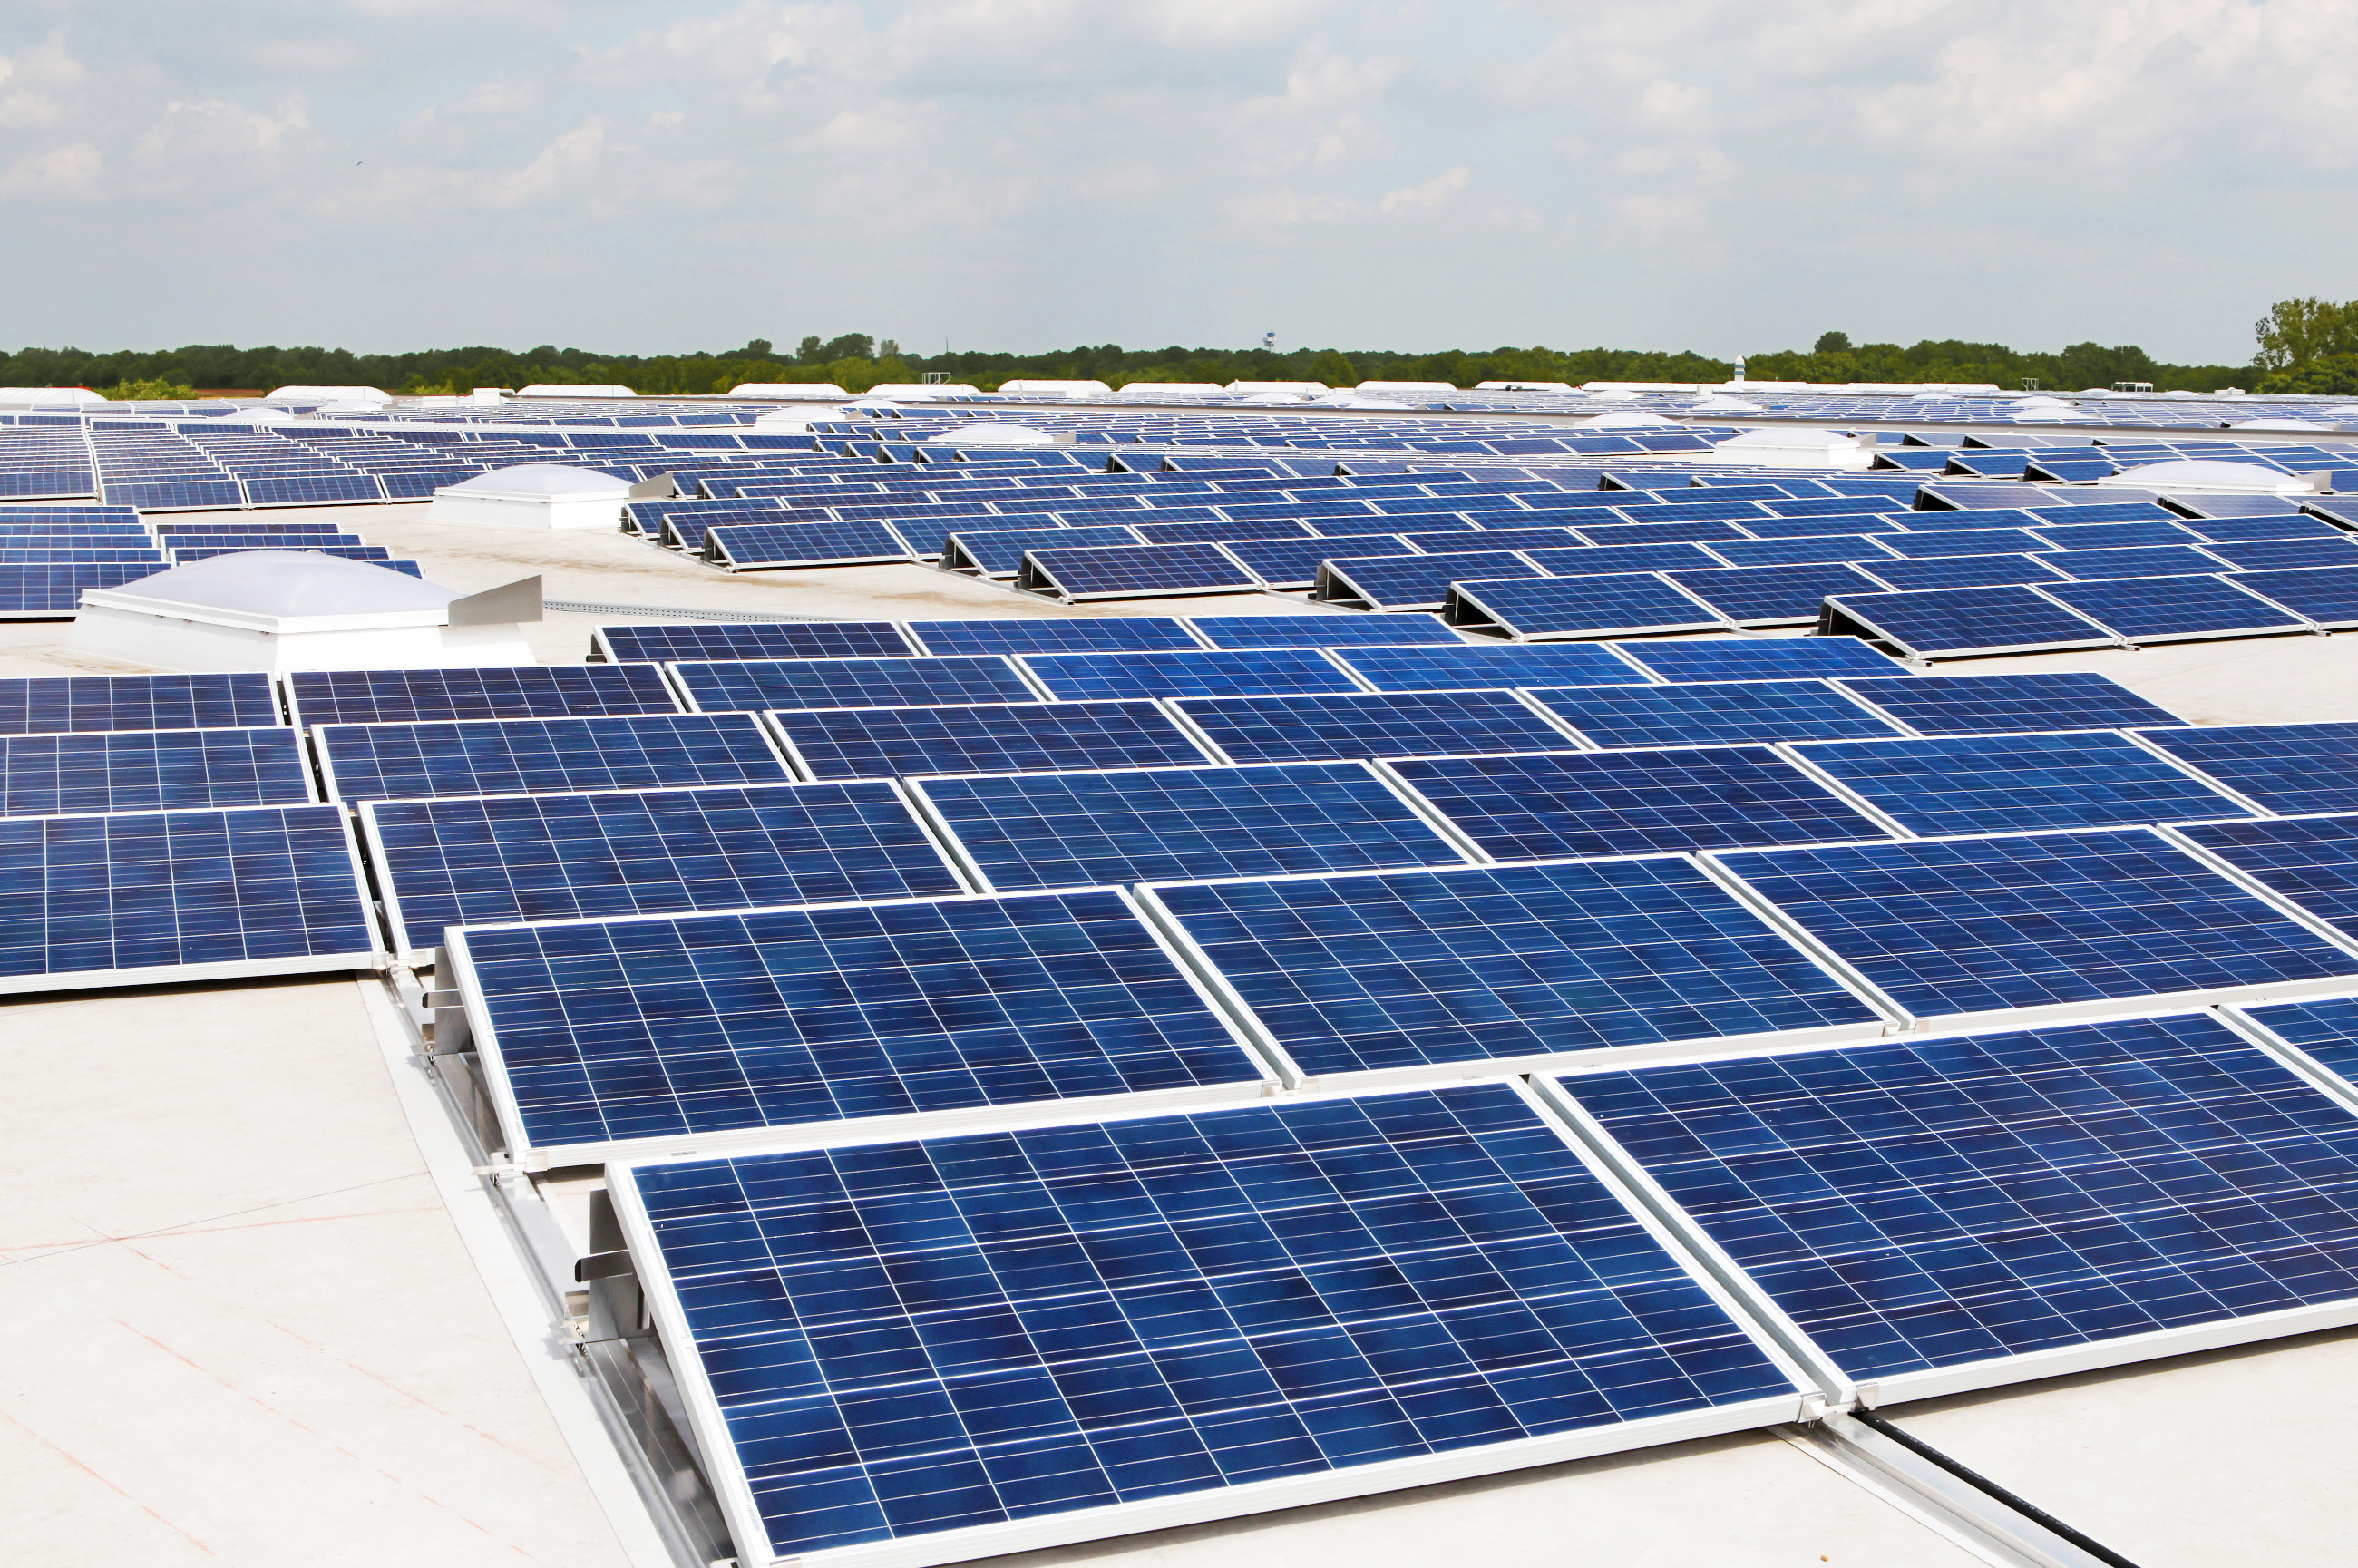
\includegraphics[width=\paperwidth,height=\paperheight]{images/titlepage/titlepic.jpg}%
        };

        % ------------------------------------------------ %
        % Info Table                                       %
        % ------------------------------------------------ %
        \node[%
            fill=black,
            fill opacity=0.75,
            rounded corners,
            outer sep=0pt,
            inner sep=1em,
            yshift=9em,
            anchor = south%
        ] at (current page.south) {\textcolor{white}{\infotable}};

        % ------------------------------------------------ %
        % FHNW Logo                                        %
        % ------------------------------------------------ %
        \node[anchor=north west,xshift=\logoX,yshift=-\logoY,outer sep=0pt,inner sep=0pt] at (current page.north west) {%
            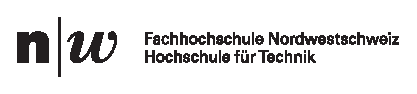
\includegraphics[height=12mm]{images/titlepage/fhnw.eps}%
        };
    \end{tikzpicture}



    % ---------------------------------------------------- %
    % The Text can  be set rather low in  the page without %
    % adjusting the top lengths.                           %
    % Backing up  and reseting these lengths  seems not to %
    % be necessary;  it appears  they are restored  at the %
    % end of the titlingpage environment.                  %
    % ---------------------------------------------------- %
    \setlength{\headsep}{0pt}
    \setlength{\headheight}{0pt}
    \setlength{\uppermargin}{4em}
    \checkandfixthelayout


    % ---------------------------------------------------- %
    % By   default,  centering   inside  the   titlingpage %
    % environment  will   center  with  respects   to  the %
    % typeblock. When  the  typeblock  is  centered,  this %
    % leads to  centered text  with respect to  the entire %
    % title  page. However,  When  the  typeblock  is  not %
    % centered, some adjustment is needed.                 %
    % See memman Chapter "Titles" for more information.    %
    % ---------------------------------------------------- %
    \calccentering{\unitlength}
    \begin{adjustwidth*}{\unitlength}{-\unitlength}


    % ---------------------------------------------------- %
    % Work some  magic to  automatically adjust  the hrule %
    % lengths to the length of the book title.             %
    %                                                      %
    % NOTE: The  font  size setting  needs  to  be in  the %
    % \mytitle  command, otherwise  \settolength will  not %
    % take it  into account  and will only  calculate with %
    % the default font size.                               %
    %                                                      %
    % NOTE  2: This mechanism  breaks if  the title  spans %
    % across multiple  lines. You're on  your own  in that %
    % case.                                                %
    % ---------------------------------------------------- %
    \newcommand{\mytitle}{{\textbf{\fontsize{25mm}{1em}\selectfont Project Powerline}}}
    \newlength{\titlelength}            % Length of title text
    \settowidth{\titlelength}{\mytitle}
    \newcommand{\titlerulefactor}{1.2}  % Length of title rules, as a factor

    % ---------------------------------------------------- %
    % Set the title color                                  %
    % ---------------------------------------------------- %
    \newcommand{\titlecolor}{black}

    % ---------------------------------------------------- %
    % Put the title onto the page                          %
    % ---------------------------------------------------- %
    \textcolor{\titlecolor}{%
        \centering
        \rule{\titlerulefactor\titlelength}{1pt} \\
        \vspace*{4mm}
        \mytitle\\
        %\vspace*{5mm}
        \rule{\titlerulefactor\titlelength}{1pt} \\
        \vspace*{6mm}
        \fontsize{8mm}{1em}\selectfont Fachbericht \\
    }


    % ---------------------------------------------------- %
    % This is the end of the centering magic.              %
    % ---------------------------------------------------- %
    \end{adjustwidth*}


    % ---------------------------------------------------- %
    % Make  sure  this  is   not  put  into  \frontmatter, %
    % otherwise it will get a \frontmatter folio.          %
    % \cleardoblepage  is not  actually necessary  because %
    % it  is  automatically   called  by  the  titlingpage %
    % environment.                                         %
    % ---------------------------------------------------- %
    %\cleardoublepage

    %\setlength{\headsep}{\originallength}
    %\checkandfixthelayout
\end{titlingpage}


% -------------------------------------------------------- %
% See  the  memoir  documentation  for  what  specifically %
% frontmatter does. Among  other things, page  numbers are %
% set to roman numerals and chapter numbers are removed.   %
% -------------------------------------------------------- %
\frontmatter

% -------------------------------------------------------- %
% Comment out what's not needed, obviously.                %
% -------------------------------------------------------- %
%\begin{centering}
\vspace*{30mm}
\begin{tiny}
    \begin{tabular}{lll}
        Inhalt & \copyright~2016 & Reto Nussbaumer   \\
               &                 &                   \\
        Design & \copyright~2016 & Raphael Frey      \\
    \end{tabular}


    % ---------------------------------------------------- %
    % Having  this  in  a  tabular  is  a  bit  ugly,  but %
    % it  ensures alignment  and  limited paragraph  width %
    % without much effort.                                 %
    % ---------------------------------------------------- %
    \vspace{1em}
    \begin{tabular}{p{.9\textwidth}}
        \noindent  Erstellt  im  Fr\"uhlingssemester 2016  an  der  Hochschule
        f\"ur  Technik  der  Fachhochschule   Nordwestschweiz  im  Rahmen  des
        Modules   \emph{Projekt  4}   des   Studiengangs  \emph{Elektro-   und
        Informationstechnologie}. \\

        \\
        \iftoggle{paper}{%
            Dies     ist    die     Druckversion    dieses     Dokuments. Eine
            elektronische     Version      mit     farbig     hervorgehobenen,
            klickbaren   Links   ist   auf  den   abgegebenen   elektronischen
            Datentr\"agern  in  Anhang \ref{app:electronicStorage}  auf  Seite
            \pageref{app:electronicStorage}   zu   finden    oder   kann   bei
            \code{raphael.frey@students.fhnw.ch} angefordert werden.
        }{%
            Dies ist die elektronische  Ausf\"uhrung des Dokuments. Links sind
            farbig hervorgehoben und klickbar. Falls eine Version ohne farbige
            Akzentuierung erw\"unscht ist, kann diese bei
            \href{mailto:raphael.frey@students.fhnw.ch}{\code{raphael.frey@students.fhnw.ch}}
            angefordert werden.
            % internet links: blau
            % externe links: magenta
        }
        \\

        \\
        Dieses Dokument hat bisher \thecounttexruns~Kompiliervorg\"ange durchlaufen. \\
    \end{tabular}
    \vspace{1em}

    \begin{tabular}{>{\ttfamily}lrl}
        Version 1 & 16.06.2016 & Abgabe \\
    \end{tabular}

    \vspace{1em}
    \begin{tabular}{l @{${}:{}$} l}
        Quelle Titelbild & \cite{ref:titlepage:pvanlage} \\
        Quelle Logo FHNW & \cite{ref:fhnwlogo}           \\
    \end{tabular}
\end{tiny}
%\\
%\footnotesize{\checkmark~\np~\noi~\partially} \\
%\\
%\large{\checkmark~\np~\noi~\partially} \\
%\\
%\checkmark~\np~\noi~\partially
%\end{centering}

%% **************************************************************************** %
\chapter*{Abstract}
\label{chap:abstract}
% **************************************************************************** %

\emph{Note: I have  added headings  for the five  sections of  the ``abstract
hand'' to  highlight my thinking process;  obviously those will be  removed in
the final version.}

\vspace{2em}
\textbf{Research Question: What does the client expect?}\\
This  project's aim  was  to  develop a  system  for  real-time monitoring  of
photovoltaic  facilities on  the level  of single  panels. The system  must be
cost-effective and should scale from small single-household solutions to large
industrial-scale solar farms. Panels which are  not operating at full capacity
for whatever reason  (dirt, shade, defects) must be detected  and announced to
the user so that appropriate measures (cleaning, replacement) can be taken.

\textbf{Relevance}\\
Monitoring individual photovoltaic modules  will allow the facility's operator
to run  their solar farm at  optimal conditions, thus reducing  losses in both
power output and money.

\textbf{Background}\\
Current solutions for per-module monitoring  of solar facilities are expensive
and are  therefore often  foregone in  order to save  costs when  building new
facilities. This approach is short-sighted and more expensive in the long term
because not being able  to properly monitor a solar facility  means that it is
often not operating at optimal  conditions. As non-renewable sources of energy
such  as fossil  fuels  and nuclear  power are  losing  ground to  alternative
sources of  energy such  as wind and  solar power, the  overall losses  in the
energy industry of power and money  incurred due to insufficient monitoring of
solar facilities will become unsustainable.

\textbf{Method}\\
Our  system consists  of  two primary  components: A  controller is  installed
centrally  near  the  inverter. Additionally,  a sensor  is  mounted  on  each
photovoltaic  panel.  Communication  between  the sensors  and  the master  is
routed  through the  direct  current power  transmission  line; no  additional
wiring is needed. A  coil is used to  couple the signal to  the power line. In
case  of  an  error (e.g.  a  dirty  panel),  a  text  message is  sent  to  a
user-configurable phone  number. Additionally, local alarms such  as sirens or
warning lights  can be connected  to our system  and are triggered  whenever a
text message is sent.

\textbf{Results}\\
Simulations for  various coupling methods  for a string  of 20 PV  panels have
been performed. Inductive  coupling at  non-resonance conditions results  in a
signal  level  of roughly  \SI{6}{\milli\volt}  peak-to-peak  at the  receiver
without  amplification. Operating  the  circuit  at resonance  yields  a  much
improved peak-to-peak  voltage of \SI{250}{\milli\volt} at  the receiver (also
without amplification), which is sufficient for our purposes.

A  frequency sweep  for  the coupling  coil has  been  measured and  inductive
behavior up to  \SI{20}{\mega\hertz} verified, thus ensuring that  the coil we
have  picked is  suitable for  our uses  and  allows the  of a  vast range  of
frequencies as  needed. The system can  therefore adapt to conditions  in each
specific setup.

\vspace{1em}
\emph{Question: How negative  should we  go in  the paragraph  below? We don't
exactly  want to  sound like  depressed failures,  but then  again, facts  are
facts, and things  just aren't working properly. Should we  also add something
about how  we would proceed if  we had the time  or is this not  the place for
that?}

\vspace{1em}
The system  in its  entirety is  at this  point not  operational. The sensor's
components  do not  yet  work perfectly  in unison;  error  analysis is  still
ongoing. The printed circuit board for the  master device is not available due
to an issue with the  manufacturer when ordering. However, development for the
master's software is mostly completed.  A functioning graphical user interface
has been implemented and a database to which it connects is functional.

\vspace{2em}
\textbf{Key  words:}  photovoltaic  technology,  photovoltaic  module,  remote
monitoring, solar technology, PV cell, power efficiency, alternative energy,
powerline, communication, inductive coupling, capacitive coupling

%\include{frontmatter/dedication}
%\include{frontmatter/declaration}
%\include{frontmatter/acknowledgements}


% -------------------------------------------------------- %
% The starred versions do not make an entry for themselves %
% in the ToC, the unstarred versions do.                   %
% -------------------------------------------------------- %
{%
\enlargethispage{4em}
\tableofcontents*
}
%\newpage\listoffigures
%\newpage\listoftables


% -------------------------------------------------------- %
% Set page numbers to  arabic numerals, reset page counter %
% to 1, display  chapter numbers. See memoir documentation %
% for more information.                                    %
% -------------------------------------------------------- %
\mainmatter


% -------------------------------------------------------- %
% It is  advisable to use actually  meaningful chapter and %
% section names instead of generically numbered ones as in %
% this  example structure. That  way, their  place in  the %
% document is not directly tied to their file name, and it %
% is  possible to  restructure the  document (e.g.  move a %
% section  from one  chapter  to another,  or reorder  the %
% chapters)  without  needing  to adjust  file  names  and %
% similar shenanigans.                                     %
% -------------------------------------------------------- %
%% **************************************************************************** %
\chapter{Einleitung}
\label{chap:einleitung}
% **************************************************************************** %

Photovoltaikanlagen   sind  heutzutage   kein   Nischenprodukt  mehr. Um   die
Abhängigkeit  vom Erdöl  zu verringern,  werden vielerorts  kleine, aber  auch
grosse  Anlagen gebaut. Die  W\"arme-Energie, welche  kostenlos von  der Sonne
kommt,  wird  in elektrische  Energie  umgewandelt  und  kann gleich  vor  Ort
genutzt werden. Anlagenbesitzer  investieren meistens einen grossen  Betrag in
eine  neue  Anlage  und  sind  darauf angewiesen,  dass  diese  den  maximalen
Ertrag  liefert. Das ist  in der  Regel  ohne grossen  Aufwand der  Fall. Doch
es  gibt Umstände,  welche  die Effizienz  einer Photovoltaikanlage  erheblich
verringern  können und  dies meist  ohne, dass  es jemand  bemerkt.  In  einer
Photovoltaikanlage  werden üblicherweise  mehrere  PV-Module  zu einem  String
zusammengefasst,  indem  sie  in   Serie  geschaltet  werden. Dabei  kann  ein
abgeschattetes,  verschmutztes  oder  gar  defektes  Modul  den  Strom  dieser
Serieschaltung und somit auch die Leistung des gesamten Strings und der Anlage
stark beeinträchtigen. Was grosse finanzielle Einbussen zur Folge haben kann.

Das  Ziel des  Projektes P4  war es,  ein PV-Überwachungssystem  bestehend aus
einer Sensorplatine für den Einbau in  die Anschlussbox jedes Moduls und einem
zentralen Meldegerät  für den Einbau  im Schaltschrank beim  Wechselrichter zu
entwickeln, aufzubauen und zu testen. Die  Sensorplatine soll die Spannung des
jeweiligen PV-Modules  messen und sie  an das Mastergerät über  die bestehende
DC-Leitung  der  Anlage  übermitteln. Im  Mastergerät  werden  die  gemessenen
Spannungen der  einzelnen PV-Module  gespeichert und  ausgewertet. Erkennt das
Mastergerät ein fehlerhaftes  PV-Modul, soll eine Alarmierung  am Gerät selbst
und  per  SMS  ausgegeben  werden. Zusätzlich wird  ein  Relais  zur  externen
Signalisation  betätigt.   Das  System  soll  möglichst  energieeffizient  und
kostengünstig sein,  um die wirtschaftlichkeit einer  Photovoltaikanlage nicht
zu verschlechtern.

Das  Hauptproblem liegt  bei  der Signalübertragung  über  die DC-Leitung  der
Photovoltaikanlage. Denn die Spannung darauf schwankt  zwischen 12 und 60 Volt
an der Sensorplatine  und beträgt am Mastergerät bis zu  1000 Volt. Auf dieser
Leitung  ein Signal  zu  übertragen  ist schwierig  und  wird heutzutage  kaum
gemacht.  Zudem muss auf kleine Leistung beim gesamten System geachtet werden,
um keine wertfolle Energie zu verschwenden.

\todo{Beschreibung unseres Produkts}

Der vorliegende  Bericht stellt  die technische Dokumentation  unseres Systems
dar.  Zuerst wird das Konzept unserer L\"osung beschrieben, zusammen mit einer
Benutzerf\"uhrung.  Anschliessend  wird auf  das Hardware-  und Firmwaredesign
eingegangen,  und   zuletzt  werden  die  am   System  durchgef\"uhrten  Tests
dokumentiert.

\lipsum



% -------------------------------------------------------- %
% Appendices are  usually numbered  and therefore  part of %
% the mainmatter, not the backmatter.                      %
% The advice about meaningful chapter names applies to the %
% appendices as well, see above.                           %
% -------------------------------------------------------- %
\appendixpage
\appendix
%% **************************************************************************** %
\chapter{\code{LTspice}-Schaltungen}
\label{app:ltspice}
% **************************************************************************** %

Dieses Kapitel  beinhaltet \code{LTspice}-Schaltungen, welche  zu Simulationen
benutzt worden sind. Erkl\"arungen  zu den jeweiligen Schaltungen  sind in den
Kapiteln  zu finden,  welche auf  sie verweisen. S\"amtliche  Schaltungen sind
auch elektronisch als \code{.asc}-Datei verf\"ugbar.

\noindent\begin{minipage}{\textwidth}
    \centering
    \includegraphics[width=0.9\textwidth]{images/ltspice/generic-iv-curves/cell.eps}
    \figcaption[\code{LTspice}-Schaltung f\"ur PV-Zelle]{%
        Modell   der   PV-Zelle,   aus   welchem  das   Modul   in   Abbildung
        \label{fig:ltspice:iv:generic:module} aufgebaut  ist. Die Simulationen
        aus   Abbildung   \ref{fig:simu:iv-curves:module:generic}  auf   Seite
        \pageref{fig:simu:iv-curves:module:generic}   basieren    auf   diesem
        Modell. Gegen\"uber     in     Abschnitt     \ref{sec:simu:model:cell}
        hergeleiteten Modell hat dieses  Modell einen h\"oheren Photostrom und
        einen niedrigeren Shunt-Widerstand. Dies  erzeugt etwas anschaulichere
        Kurven.%
    }
    \label{fig:ltspice:iv:generic:cell}
    \includegraphics[width=0.9\textwidth]{images/ltspice/jac/cell.eps}
    \figcaption[\code{LTspice}-Schaltung f\"ur PV-Zelle]{%
        Modell  der   PV-Zelle,  auf  welchen  die   Simulationen  in  Kapitel
        \ref{chap:simu} ab  Seite \pageref{chap:simu}  beruhen. Die Herleitung
        ist in Abschnitt \ref{sec:simu:model:cell} dokumentiert.%
    }
    \label{fig:ltspice:jac:cell}
\end{minipage}

\begin{figure}[h!tb]
    \centering
    \begin{tikzpicture}[%
        spy scope = {magnification=7,size=25*8,connect spies},
        every spy on node/.style={circle,red,draw},
        every spy in node/.style = {circle, fill=white, fill opacity=1, draw},
        ]
        \node[inner sep = 0pt,anchor=south west] {%
            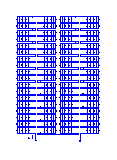
\includegraphics[width=\textwidth]{images/ltspice/generic-iv-curves/module.eps}
        };
        \spy[red] on (0.45,1.2) in node at (10,8);
    \end{tikzpicture}
    \caption[\code{LTspice}-Schaltung f\"ur PV-Modul f\"ur IV- und PV-Kurven]{%
        \code{LTspice}-Modell,    welches    zur    Erzeugung    der    Kurven
        in   Abbildung   \ref{fig:simu:iv-curves:module:generic}   auf   Seite
        \pageref{fig:simu:iv-curves:module:generic}  benutzt  worden  ist. Das
        Modell  der Zelle,  aus welcher  dieses  Modul aufgebaut  ist, ist  in
        Abbildung \ref{fig:ltspice:iv:generic:cell} abgebildet.%
    }
    \label{fig:ltspice:iv:generic:module}
\end{figure}

\begin{figure}[h!tb]
    \centering
    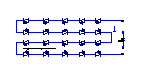
\includegraphics[width=\textwidth]{images/ltspice/jac/stringNoD.eps}
    \caption[\code{LTspice}-Schaltung f\"ur Modulstrang]{%
        \code{LTspice}-Schaltung  f\"ur  einen   Modulstrang  aus  20  Modulen
        und   variablem  Lastwiderstand   \code{Rload}   zur  Erstellung   von
        Strom-Spannungs-Kurven. Es  wird   je  ein  Strang  aus   Modulen  mit
        Freilaufdiode   (Abbildung  \ref{fig:ltspice:jacModule:NoDiode})   und
        ohne   Freilaufdiode   (Abbildung   \ref{fig:ltspice:jacModule:Diode})
        simuliert.%
    }
    \label{fig:ltspice:string:ivCurve}
\end{figure}

\begin{figure}[h!tb]
    \centering
    \begin{tikzpicture}[%
        spy scope = {magnification=5,height=25*5.5,width=25*10,connect spies},
        every spy on node/.style={rectangle,red,draw},
        every spy in node/.style = {rectangle,fill=white, fill opacity=1, draw},
        ]
        \node[inner sep = 0pt,anchor=south west] {%
            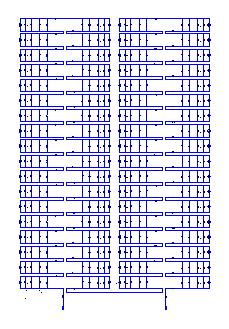
\includegraphics[width=\textwidth]{images/ltspice/jac/jacModuleNoD.eps}
        };
        \spy[red] on (1.15,1.13) in node at (9,8);
    \end{tikzpicture}
    \caption[\code{LTspice}-Schaltung f\"ur PV-Modul ohne Freilaufdiode]{%
        Modul    ohne   Freilaufdiode,    benutzt    f\"ur   die    Simulation
        aus   Abbildung   \ref{fig:simu:iv-curves:array:generic}   von   Seite
        \pageref{fig:simu:iv-curves:array:generic}.%
    }
    \label{fig:ltspice:jacModule:NoDiode}
\end{figure}

\begin{figure}[h!tb]
    \centering
    \begin{tikzpicture}[%
        spy scope = {magnification=5,height=25*5.5,width=25*10,connect spies},
        every spy on node/.style={red,draw},
        every spy in node/.style = {fill=white, fill opacity=1, draw},
        ]
        \node[inner sep = 0pt,anchor=south west] {%
            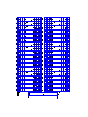
\includegraphics[width=\textwidth]{images/ltspice/jac/jacModule.eps}
        };
        \spy[rectangle,red] on (1.15,1.13) in node at (9,8);
        \spy[circle,size=25*3,red] on (7.05,0.9) in node at (9,3);
    \end{tikzpicture}
    \caption[\code{LTspice}-Schaltung f\"ur PV-Modul mit Freilaufdiode]{%
        Modul      mit      Freilaufdiode       (unten,      Mitte,      Diode
        \code{D145}). Benutzt       f\"ur       die       Simulation       aus
        Abbildung   \ref{fig:simu:iv-curves:array:generic:bypass}  von   Seite
        \pageref{fig:simu:iv-curves:array:generic:bypass}       sowie      die
        Simulationen zu den L\"osungsvarianten in Abschnitt
        \ref{sec:simu:coupling:inductive} ab Seite
        \pageref{sec:simu:coupling:inductive}, Abschnitt
        \ref{sec:simu:coupling:capacitive} ab Seite
        \pageref{sec:simu:coupling:capacitive} und Abschnitt
        \ref{sec:simu:short} ab Seite
        \pageref{sec:simu:short}.
        Abbildung   \ref{fig:ltspice:jac:cell}    enth\"alt   das   verwendete
        Zellenmodell.%
    }
    \label{fig:ltspice:jacModule:Diode}
\end{figure}

%% **************************************************************************** %
\chapter{Kosten}
\label{app:costs}
% **************************************************************************** %

%% **************************************************************************** %
\chapter{Elektronische Datentr\"ager}
\label{app:electronicStorage}
% **************************************************************************** %



% -------------------------------------------------------- %
% Page  numbering continues,  but chapter  numbers are  no %
% longer  displayed. See  memoir  documentation  for  more %
% information.                                             %
% -------------------------------------------------------- %
\backmatter

% -------------------------------------------------------- %
% Bibliography: We  are using  the  IEEEtran package  from %
% Michael Shell                                            %
%                                                          %
% There  are  a  few  different  styles  in  the  IEEEtran %
% package.   We are  going to  use  one of  two of  those, %
% either in the sorted or unsorted variety.                %
%                                                          %
% The sorted  version sorts  bibliographic entries  in the %
% bibliography alphabetically, while  the unsorted version %
% lists bibliographic  entries in the order  in which they %
% were cited (first occurrence).                           %
% -------------------------------------------------------- %
%\bibliographystyle{bibliography/IEEEtranS} % sorted
\raggedright
\bibliographystyle{bibliography/IEEEtran} % unsorted
\bibliography{bibliography/references}
\end{document}
